\documentclass[a4paper]{article}

\usepackage[english]{babel}
\usepackage[UKenglish]{isodate}
\usepackage[parfill]{parskip}
\usepackage{algorithm}
\usepackage{algpseudocode}
\usepackage{float}
\usepackage{graphicx}
\usepackage{booktabs}
\usepackage{csquotes}
%\usepackage[margin=2.5cm]{geometry}
\usepackage{listings}
\usepackage{enumerate}
\usepackage{siunitx}
\usepackage{amssymb}
\usepackage{amsthm}
\usepackage{mathtools}
\usepackage{appendix}
\usepackage[style=ieee,
            natbib=true,
            backend=biber]{biblatex}

\addbibresource{references.bib}
\usepackage[hidelinks]{hyperref}
\nocite{*}

\DeclarePairedDelimiter{\ceil}{\lceil}{\rceil}
\DeclarePairedDelimiter{\floor}{\lfloor}{\rfloor}

\newcommand\ddfrac[2]{\frac{\displaystyle #1}{\displaystyle #2}}

\newcommand{\nth}{\textsuperscript}
\renewcommand*{\arraystretch}{1.3}

\newtheorem*{lemma}{Lemma}
\newtheorem*{theorem}{Theorem}

\title{Modifying Markov Chains to Model Traffic}
\author{Kevin Zihong Ni\\\texttt{z5025098}}

\begin{document}

\maketitle

\begin{abstract}
	In this paper, we will describe the modification and adaptation of a traditional discrete time Markov Chain to efficiently model how 
	traffic jams evolve based on the live traffic conditions of every road in a network.
	We will show how this model performed experimentally with respect to both accuracy and time.
\end{abstract}

\section{Introduction}
Vehichular route planning is an important service in the software industry, being provided by various companies such as Google, Apple and Uber.
Some of these services collect live traffic data through the gps units in the smartphones of drivers.
This data is used to improve route planning, choosing routes to avoid high traffic areas.
However, traffic conditions in a road network changes over time and areas that are currently experiencing high traffic may clear up over the next minutes and vice versa.
This is problematic for route planning over long distances, 
as an algorithm may produce a route that goes around an existing traffic jam which would have cleared by the time the driver had reached it.  
It is apparent how traffic forecasting systems could be of benefit to these routing algorithms.

While it is possible to predict, with relative accuracy, the conditions of roads based on historical data, 
these models break down in abnormal traffic conditions that may be caused by external events such as accidents or roadworks.
The model this paper explores uses a combination of historical and live traffic data in order to make short to medium term forecasts that take into account any 
abnormal conditions. 

\section{Model}
While the behaviour of individual cars on the street are highly unpredictable (without the knowledge of its intended destination), we notice that the collective behaviour 
of all cars in a road network becomes very predictable.
By this, we mean that the traffic conditions of the entire network is highly dependent on the traffic conditions of the network a few moments in the past.
This is an area which lends itself to Markov Chains well, as shown by previous uses of the technique such as modelling demographic shift.
Markov chains model the changes in the states between discrete timesteps. 
Hence, before we define our model, we must first declare how much real world time (in seconds) does one timestep represent. 
Let this timestep be $t$.

\subsection{Topology}
We assume we are given a set of roads $E$ and a set of intersections $V$ together making a directed graph $G = (V, E)$.
Every edge $e \in E$ also has a length in meters $d(e)$ and a speed in meters per second $s(e)$ associated with it.
For simplicity, we also assume that $G$ has no self loops or parallel edges. These features can be trivially added to the model if necessary.

We also make the reasonable assumption that $G$ is strongly connected.
This can be done as the alternative implies either one of the following statements:
\begin{itemize}
	\item There are more than one connected components in which case we can create a separate model for each component.
	\item There are more than one strongly connected components which implies that there are places in the network which 
		a vehichle can enter but never leave (or vice versa) which is clearly absurd.
\end{itemize}

The states of our Markov chain will simply be the set of edges $E$, since this is where the overwhelming majority of cars will be at any one time.

\subsubsection{Road Based Graph}
Since the vertices of the graph represented by a Markov Matrix will become the states of that respective Markov Chain, it is necessary to 
transform our intersection based graph $G$ into another, road based graph $G' = (E, T)$ as outlined by \cite{volk}. 
$T$ denotes the set of possible "turns" in $G$, i.e. the set of possible transitions from one road to another.
An example of this transformation is illustrated in figures \ref{fig:int} and \ref{fig:roa}.

\begin{figure}[h]
    \centering
    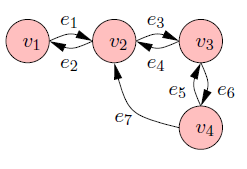
\includegraphics[width=0.4\textwidth]{intersection.PNG}
    \caption{intersection based graph}
    \label{fig:int}
\end{figure}

\begin{figure}[h]
    \centering
    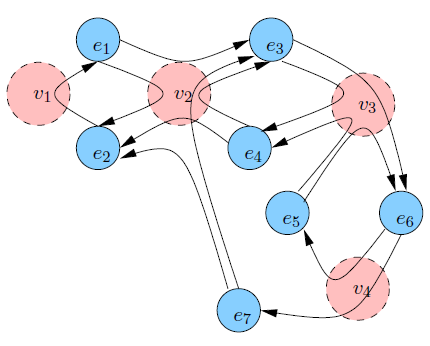
\includegraphics[width=0.7\textwidth]{road.PNG}
    \caption{road based graph}
    \label{fig:roa}
\end{figure}

\subsubsection{Turn Weights}
We also must assign a weight to each turn $t \in T$. 
This weight will be used as the (base) transition probability in the markov chain. 
When calculating these weights, we assume that their destinations has the capacity to accept an infinite number of cars. 
This number will be fixed to accomadate these road capacities later.
First, we will need to determine what fraction of cars in each road $e \in E$ will leave $e$ in each timestep. 
We define this to be
$$
l(e) = \min \left(1, \ddfrac{t \epsilon s(e)}{d(e)} \right)
$$

where $\epsilon$ is a constant that accounts for small losses in efficiency due to turning and unexpected changes in speed.

We now consider the edges that $e$ is connected to. The combined weights of all turns to these edges must total $l(e)$.
The simplest solution to this would be to just assign $l(e)/\mathrm{outdegree}(e)$ to each turn.
However, here we also have an opportunity to incorporate historical data into our model.
Provided we have the empirical data showing the number of different turns made at each likelihood 
(which should be trivial to implement with mobile phone live traffic collection), we can calculate the relative likelihood of a turn out of $e$ to each turn $e'$, $P(e, e')$.
The weight of the turn $(e, e')$ will then be $P(e, e') l(e)$.

Putting this all together, we can construct $T$ with the following algorithm
\begin{algorithmic}[1]
	\Function{FindTurns}{$G$}
		\State $T \gets \varnothing$
		\For{$v \in V$}
			\For{$e \in \mathrm{incoming}(v)$}
				\For{$'e \in \mathrm{outgoing}(v)$}
					\State $T \gets T \cup \{(e, e', P(e, e') l(e))\}$
				\EndFor
			\EndFor
		\EndFor
		\State return $T$
	\EndFunction
\end{algorithmic}

\subsection{State Transitions}
We define the current state of the road network as a row vector $\mathbf{v}$ where $v_i$ is an estimation of the number of cars on road $i$.
Our algorithm will take the original state of the network $\mathbf{v}^{(0)}$ as input.
To step this model forward in time, we will use a similar approach to that of a Markov Chain model --- 
that is, we determine each subsequent state vector $\mathbf{v}^{(k + 1)}$ by multiplying the
preceding vector $\mathbf{v}^{(k)}$ with a transition matrix.

One naive solution would be to simply be use the adjacency matrix of $G'$ for this.
While this may suffice for low density traffic, a number of problems arise as the capacities of individual roads fill up.
\begin{itemize}
	\item In this model, there is no theoretical limit on how many cars roads can accumulate.
		We would ideally want to have a hard limit on each road $e$ proportional to $l(e)$.
	\item Each road has no limit of cars it can "accept" in one timestep, wheras it should be limited to a constant.
	\item The speed of traffic in the model is not at all affected by the density of the traffic when in reality, the speed should slow down in high traffic conditions.
\end{itemize}

We can address all these problems simultaneously by creating our transition matrix $M^{(k)}$ based on $\mathbf{v}^{(k)}$ such that these limits are respected.
From there we can determine 
$$\mathbf{v}^{(k + 1)} = M^{(k)}\mathbf{v}^{(k)}$$

\subsection{Transition Matrix}
First we define $M^B$ to be our adjacency matrix of $G'$. This matrix represents the flow of vehichles in the network if there was no loss of efficiency due to traffic.
We also need to define a vector $\mathbf{c}$ which represents the capacities of each road. For each road $e$,
$$
\mathbf{c}_e = \frac{l(e)}{\mathrm{cargap}}
$$
where cargap is a constant representing the average gap between stationary cars (including the body of the leading car). In our experiments we used cargap = 8.

All what we have described so far need only be calculated once during initialisation. To construct $M^{(k)}$ given $\mathbf{v}^{(k)}$, we first must calculate
$\mathbf{h}^{(k)} = M^B \mathbf{v}^{(k)}$. This vector represents the maximum flow of traffic, given ideal conditions.
we aim to construct $M^{(k)}$ by reducing the weights of $M^B$ based on $\mathbf{h}^{(k)}$ and $\mathbf{v}^{(k)}$. We need to calculate a "limit" vector, $\mathbf{l}^{(k)}$, where
$\mathbf{l}^{(k)}_e$ is the maximum number of cars that can be accepted by road $e$ in the next timestep.
For each road $e$, to impose a limit on the input capacity, we need to keep $\mathbf{l}^{(k)}_e \leq t/g$,
where $g$ is the "time gap" between vehichles in seconds --- that is, at a fixed point on the road, what is the minimum amount of time after the previous car passing until the next car passes (we used $g = 3$ in our experiments).
To impose a limit on the total capacity, we also need to keep $\mathbf{l}^{(k)}_e \leq \mathbf{c}_e - \mathbf{v}^{(k)}_e$.

We take the min of these two values, resulting in

$$\mathbf{l}^{(k)}_e = \min \left(\frac{t}{g}, \mathbf{c}_e - \mathbf{v}^{(k)}_e \right)$$

The ratios that we need to reduce each column of $M^B$ by can be found by taking the elementwise division of $\mathbf{l}^{(k)}$ and $\mathbf{v}^{(k)}$,
and taking the min of each element and 1. To apply these ratios to $M^B$, we construct a diagonal matrix $R^{(k)}$ such that 
$$
R^{(k)}_{e, e} = \min\left(\frac{\mathbf{l}^{(k)}_e}{\mathbf{v}^{(k)}_e}, 1 \right)
$$
Our change matrix can then be defined as
$$
C^{(k)} = M^B R^{(k)}
$$

Lastly, we need to make our matrix stochastic. To do this, we find the difference between the sum of each row and 1
$$
\mathbf{d}^{(k)} = \mathbf{e} - C^{(k)} \mathbf{e}
$$
where $\mathbf{e}$ is a row vector of length $|E|$ filled with ones.
This vector represents the "discrepancy" in each row of $C{(k)}$. We will resolve this discrepancy by adding $\mathbf{r}^{(k)}$, to the diagonal of $C^{(k)}$, representing
the cars in that road that remain in the same road for the duration of the timestep.

Hence, if we define a matrix $D^{(k)}$ such that $ D^{(k)}_{e, e} = \mathbf{d}^{(k)}_e $ then

$$M^{(k)} = C^{(k)} + D^{(k)}$$

\section{Evaluation}
\subsection{Time and Memory}
Since the matrices we are working with are sparse (elements are predominatly zeroes), The memory complexity of the algorithm is $O(|T|)$, since we only need to keep track of
the non zero entries of the matrix. Likewise, the matrix multiplications are also significantly faster compared to those of dense matrices, with each multiplication 
(with a vector) running in $O(|T|)$. 

Due to the highly "vectorised" definition of the algorithm, we can take advantage of existing, highly optimised linear algebra libraries; speeding up implementation and
improving performance.

\subsubsection{Performance Tests}
Our tests ran on a computer with a Intel(R) Core(TM) i5-4670 CPU running at a clock speed of 3.4 GHz and 16 GB of RAM.
We ran the algorithm for 3600 cycles over the Australian road network provided by PitneyBowes StreetPro v2015. 
This network had $|N| = 3162911$, $|E| = 4001065$ and $|T| = 9407137$.
No multithreading was used. 

Our algorithm ran in $5681.56690120697$
seconds, with an average of $1.57821302811$
seconds per cycle. The program used less than 2GB of memory after initialization.

\subsection{Accuracy}
We chose to use the unchanged initial states as the baseline for our model, since this is the existing estimation that our model seeks to replace.
We also evaluated how $t$ affects the accuracy of our model by running our model with it set to different values.
Finally we wanted to see how the accuracy of our model deteriorates over time. 

These tests were done under with the road network in two different conditions --- once where there was a major traffic jam and another under normal traffic conditions.

\subsubsection{Accuracy Test Data Synthesis}
Lacking real life data to evaluate our model against, we instead created synthetic data by simulating the movement of cars in the road network.
We did this by keeping track of the locations of $n$ different "cars" in the network. 
The original positions were initialised according to a gaussian distribution around a certain point in the network.
When emulating a traffic jam, the standard deviation of this distribution was set very low, causing the cars to be generated very close to the selected point.
When emulating regular traffic, the standard deviation of this distribution was set close to half of the radius of the selected area,
causing the cars to be relatively uniformly.
These cars performed a random walk around the network based on the predetermined turn probabilities. %TODO

To introduce the road capacities to the network, we keep track of a "fullness" function $c(e)$ where $c(e)$ is the "apparent fullness" of $e$.
By "apparent fullness", we mean how "full" a road appears from an observer at the "mouth" of the road trying to turn into it. This may possibly be greater than
the number of cars actually in $e$, since, in a queue, human driven cars don't accelerate in unison but only accelerate after the car ahead of it starts to accelerate.
This may cause gaps in the road that propagate backwards as cars move forwards to fill the gap.
In addition, we use a system of 3 priority queues, all containing and ordered by a "time" value --- that is, the
simulated time where the "event" that the queue entry is tracking takes place.
\begin{enumerate}
	\item A priority queue to keep track of cars in the middle of roads and when they will reach the next intersection. Each time a car comes off this queue, we append it
		to a "waiting list" queue of the road that it is moving to (but we do NOT move it yet).
	\item A priority queue to keep track of "gaps" in roads caused by cars leaving the road at the end and when they (the gaps) will reach the beginning of the road. 
		Each time a road $e$ comes off this queue, we decrement $c(e)$, allowing for more cars to enter.
	\item Each road must be locked for $g$ seconds after a car enters it in order to enforce a minimum gap between cars. Our third queue simply
		keeps track of when these roads become unlocked.
\end{enumerate}

To run this simulation, we would take the earliest event in all 3 of these queues (however we only need to check the top of the queues since they are all min queues), and
process it accordingly.
Each time we do this, we need to check the "waiting list" queues of the appropriate road $e$ 
(the road that the car is moving to for queue 1 and road in the queue entry for queues 2 and 3), and if it is not locked or at capacity, we move the car 
into $e$.

Each time a car $k$ successfully moves from a old road $e$ into a new road $e'$ at time $t$, in addition to incrementing $c(e)$, 
we would also need to create appropriate new entries for the aforementioned queues.
\begin{enumerate}
	\item Add an entry to queue 1, containing $k$ with time value $t + d(e')/s(e')$.
	\item Add an entry to queue 2, containing $e$ with time value $t + r * c(e)$, and $r$ 
		is a constant representing the average time it takes for a driver to start
		moving once the cars ahead of it start to move. We used $r = 2$.
	\item Add an entry to queue 3, containing $e'$ with time value $t + g$.
\end{enumerate}

This simulation ran considerably slower than our Markov chain model and so we only tested a small subset of the road network, including areas within the Greater Sydney Metro 
area. This smaller network had $|N| = 16443$, $|E| = 22639$ and $|T| = 81451$.

We would run this simulation for an amount of simulated time and record the number of cars in each road at specified checkpoints.
These checkpoints can then be used to evaluate our model by taking a certain checkpoint as an input vector, step it through time using the model and compare the resulting
state of the network to later checkpoints.
For our evaluation, we ran the simulation for an hour of simulated time and recorded a checkpoint at every minute.


\subsubsection{Results}
For all of our tests, We set our error value to be the euclidean distance between our current state vector and the target state vector (the L2 norm).
Our results are as shown in figures \ref{fig:acc} and \ref{fig:reg} for traffic jam and regular traffic scenarios respectively (generated by matplotlib).

\begin{figure}[H]
    \centering
    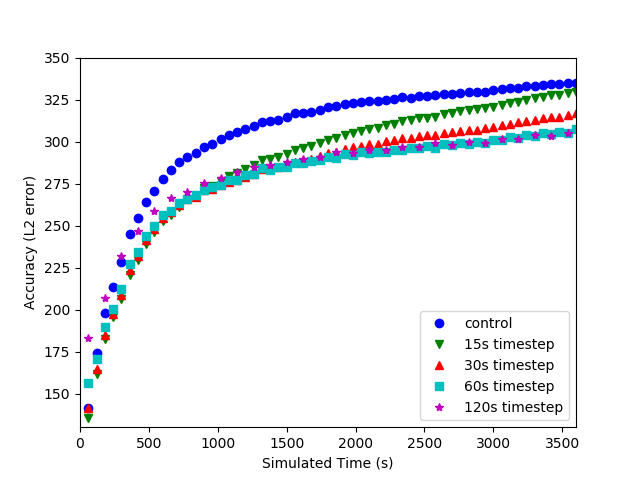
\includegraphics[width=1\textwidth]{Results.png}
	\caption{Accuracy of different models in a traffic jam}
    \label{fig:acc}
\end{figure}

In terms of mid range accuracy, our model performs noticably better than the control in all cases with larger values of $t$ producing more accurate results.
This advantage tapers off after $t = 60$. This can be attributed to models with longer timesteps being more "stable"; since models with smaller $t$ must perform 
more multiplications to step forward a certain amount of time, allowing for more opportunities for errors to compound.

\begin{figure}[H]
    \centering
    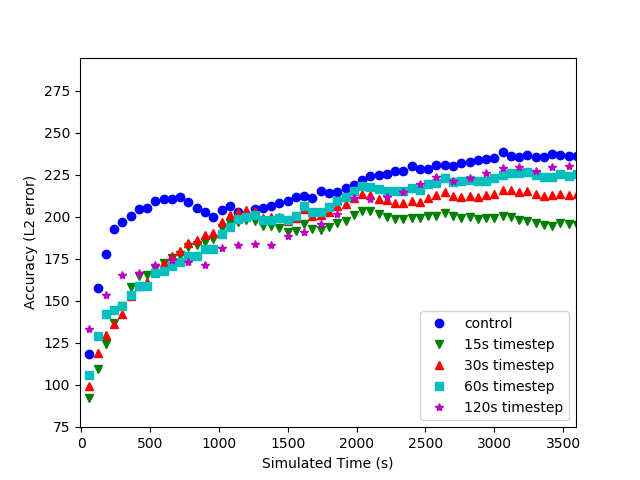
\includegraphics[width=1\textwidth]{Results2.png}
	\caption{Accuracy of different models in regular traffic}
    \label{fig:reg}
\end{figure}

While the results of our model still remains better than that of the control, an increase in $t$ now has an opposite effect to the traffic jam tests.

One source of inaccuracy for high $t$ models is the fact that, in one timestep, they can at most only model the movement of cars into roads immediately adjacent to the ones
that they are currently in.
This becomes an issue when traffic flow is efficient, as cars may have moved to a road that are at higher degrees of separation within a span of a timestep.
While this issue obviously also exists in low $t$ models, it is far less prevalent since cars will not be able to travel as far in that shorter timespan.
This may explain our results as, when roads are saturated, traffic moves considerably more slowly and thus the main source of errors in high $t$ models are mitigated.

\printbibliography
\end{document}
